\chapter{The Second Moment}

\lecture{8}{20 Oct.}{}

Everything so far has been an existence argument. The union bound and \autoref{lem:first-moment} both end with the words \emph{there is an \(\omega\) with\dots}, and the method of alterations repaired a single such \(\omega\) by hand. None of this says anything about how a \emph{typical} outcome looks.

This chapter changes that. Knowing \(\mathbb{E}[X]\) alone, one cannot tell whether \(X\) is usually close to its mean or wildly spread out; the variance is what distinguishes the two, and it is cheap to compute for the sums of indicators that keep appearing in our applications.

\begin{moral}
    The first moment finds one good outcome. The second moment shows that \emph{almost every} outcome is good: if \(\Var(X)\) is small compared with \(\mathbb{E}[X]^2\), then \(X\) is concentrated around \(\mathbb{E}[X]\).
\end{moral}

From this chapter on the statements are asymptotic, so it is worth fixing once and for all what the limits are taken in.

\begin{notation}[Asymptotics]
    All objects come in sequences indexed by a parameter \(n \to \infty\): a probability space \((\Omega_n, \mathbb{P})\), a random variable \(X_n\) on it, and events \(A_n \subseteq \Omega_n\). Every Landau symbol --- \(o\), \(O\), \(\Theta\), \(\ll\), \(\gg\) --- refers to \(n \to \infty\), and every other parameter (\(k\), \(\ell\), \(\varepsilon\), \(c\), \dots) is a constant held fixed as \(n\) grows. Thus:
    \begin{itemize}
        \item \(\mathbb{E}[X_n] = o(1)\) means \(\mathbb{E}[X_n] \to 0\) as \(n \to \infty\);
        \item \(A_n\) holds \vocab{with high probability} if \(\mathbb{P}(A_n) \to 1\) as \(n \to \infty\);
        \item \(X_n = (1 + o(1)) \mathbb{E}[X_n]\) with high probability means: for every fixed \(\varepsilon > 0\),
        \[
            \mathbb{P}\Bigl( \abs{X_n - \mathbb{E}[X_n]} \le \varepsilon \, \mathbb{E}[X_n] \Bigr) \longrightarrow 1 .
        \]
        Note the order of the quantifiers: \(\varepsilon\) is chosen first and the probability tends to \(1\) for that \(\varepsilon\); the rate may depend on \(\varepsilon\).
    \end{itemize}
    As usual we suppress the subscript and write \(X\) for \(X_n\), since in the applications the dependence on \(n\) is visible anyway --- \(X\) counts triangles in \(G(n,p)\), and \(p = p(n)\).
\end{notation}

\section{Markov's and Chebyshev's Inequalities}\label{sec:markov-chebyshev}

\subsection{One Tail from the Mean Alone}

\autoref{lem:first-moment} says that \(\{X \le \mathbb{E}[X]\}\) has positive probability, so a small expectation forces some outcome to be small. Markov's inequality is the quantitative version: for a non-negative \(X\), knowing only \(\mathbb{E}[X]\) already limits how much mass can sit far out on the right.

\begin{theorem}[Markov's inequality]\label{thm:markov}
    Let \(X \ge 0\) be a random variable. Then for every \(a > 0\),
    \[
        \mathbb{P}(X \ge a) \le \frac{\mathbb{E}[X]}{a}.
    \]
\end{theorem}

\begin{proof}
    Take \(X\) discrete. Splitting the defining sum at \(a\) and discarding the small values,
    \[
        \mathbb{E}[X]
        = \sum_{x} x \, \mathbb{P}(X = x)
        = \sum_{x < a} x \, \mathbb{P}(X = x) + \sum_{x \ge a} x \, \mathbb{P}(X = x)
        \ \ge\ \sum_{x < a} 0 \cdot \mathbb{P}(X = x) + \sum_{x \ge a} a \, \mathbb{P}(X = x),
    \]
    where the first sum was dropped using \(X \ge 0\) and the second bounded using \(x \ge a\). The right-hand side is \(a \, \mathbb{P}(X \ge a)\), and dividing by \(a\) gives the claim.
\end{proof}

\begin{eg}[First moment, restated]\label{eg:markov-first-moment}
    Let \(X \ge 0\) be integer-valued, as it is whenever \(X\) counts something. Taking \(a = 1\) in \thmref{thm:markov} gives
    \[
        \mathbb{P}(X \ge 1) \le \mathbb{E}[X],
        \qquad\text{equivalently}\qquad
        \mathbb{P}(X = 0) \ge 1 - \mathbb{E}[X],
    \]
    and this is how we have been using the first moment all along. The two readings of it differ in exactly the way the chapter is about.
    \begin{itemize}
        \item \emph{One space, no limit.} If \(\mathbb{E}[X] < 1\) then \(\mathbb{P}(X = 0) > 0\), so there exists an outcome with \(X = 0\). This is the existence statement of the previous chapters, and nothing is tending to anything.
        \item \emph{A sequence, \(n \to \infty\).} If \(X = X_n\) is a sequence as in the convention above and \(\mathbb{E}[X_n] = o(1)\), then \(\mathbb{P}(X_n = 0) \ge 1 - \mathbb{E}[X_n] \to 1\), i.e.\ \(X_n = 0\) with high probability. This is a statement about almost all outcomes, not just one.
    \end{itemize}
\end{eg}

\subsection{A Large Mean Says Nothing}

The other direction fails completely.

\begin{question}\label{q:large-mean}
    If \(\mathbb{E}[X]\) is large, is \(X\) large with high probability?
\end{question}

\begin{proof}[Answer]
    No. For a single space, let
    \[
        X = \begin{cases}
            10^{6}, & \text{with probability } \frac{1}{1000}, \\
            0, & \text{with probability } \frac{999}{1000},
        \end{cases}
    \]
    so that \(\mathbb{E}[X] = 1000\) while \(X = 0\) with probability \(0.999\): the mean is carried entirely by a rare enormous value.

    To say this asymptotically, take the same example with \(n\) in place of \(1000\): let
    \[
        X_n = \begin{cases}
            n^{2}, & \text{with probability } \frac{1}{n}, \\
            0, & \text{with probability } 1 - \frac{1}{n}.
        \end{cases}
    \]
    Then \(\mathbb{E}[X_n] = n \to \infty\), and yet \(\mathbb{P}(X_n > 0) = \frac{1}{n} \to 0\), i.e.\ \(X_n = 0\) with high probability.
\end{proof}

So \(\mathbb{E}[X_n] \to \infty\) does \emph{not} give \(\mathbb{P}(X_n > 0) \to 1\); the example shows it does not even prevent \(\mathbb{P}(X_n > 0) \to 0\). To rule out this behavior we need to know that \(X_n\) does not spread out, which is what the second moment measures.

\subsection{Chebyshev's Inequality}

\begin{theorem}[Chebyshev's inequality]\label{thm:chebyshev}
    Let \(X\) be a random variable and let \(a > 0\). Then
    \[
        \mathbb{P}\bigl( \abs{X - \mathbb{E}[X]} \ge a \bigr) \le \frac{\Var(X)}{a^{2}}.
    \]
\end{theorem}

\begin{proof}
    The random variable \((X - \mathbb{E}[X])^{2}\) is non-negative and has expectation \(\Var(X)\), so \thmref{thm:markov} applies to it with threshold \(a^{2}\):
    \[
        \mathbb{P}\bigl( (X - \mathbb{E}[X])^{2} \ge a^{2} \bigr)
        \le \frac{\mathbb{E}\bigl[ (X - \mathbb{E}[X])^{2} \bigr]}{a^{2}}
        = \frac{\Var(X)}{a^{2}}.
    \]
    Finally, since \(a > 0\), the event on the left is literally the event \(\abs{X - \mathbb{E}[X]} \ge a\).
\end{proof}

\begin{remark}\hfill
    \begin{enumerate}[(1)]
        \item Write \(\sigma \coloneqq \sqrt{\Var(X)}\) and put \(a = \lambda \sigma\), i.e.\ measure the deviation in units of \(\sigma\):
        \[
            \mathbb{P}\bigl( \abs{X - \mathbb{E}[X]} \ge \lambda \sigma \bigr)
            \le \frac{\Var(X)}{(\lambda \sigma)^{2}}
            = \frac{1}{\lambda^{2}}.
        \]
        This holds for every \(\lambda > 0\), with no limit taken anywhere; it is the form in which Chebyshev's inequality is usually stated.

        To read it asymptotically, let \(\lambda = \lambda(n) \to \infty\) arbitrarily slowly. Then \(\lambda(n)^{-2} \to 0\), so
        \[
            \mathbb{P}\Bigl( \abs{X - \mathbb{E}[X]} < \lambda(n) \, \sigma \Bigr) \longrightarrow 1 .
        \]
        That is, a random variable is unlikely to be \(\omega\bigl( \sqrt{\Var(X)} \bigr)\) away from its expectation.
        \item Chebyshev can also beat Markov on the \emph{upper} tail. For \(a \gg \mathbb{E}[X]\),
        \[
            \mathbb{P}(X \ge a) \le \mathbb{P}\bigl( \abs{X - \mathbb{E}[X]} \ge a - \mathbb{E}[X] \bigr) \le \frac{\Var(X)}{(a - \mathbb{E}[X])^{2}},
        \]
        which decays like \(a^{-2}\) rather than Markov's \(a^{-1}\). Whenever \(\Var(X)\) is not much bigger than \(\mathbb{E}[X]\) --- and \autoref{lem:variance-indicators} below says this is the typical situation --- the second bound is the stronger one.
    \end{enumerate}
\end{remark}

\section{The Variance of a Sum of Indicators}\label{sec:variance-indicators}

To use \thmref{thm:chebyshev} we must be able to compute, or at least bound, variances. In every application we have met, the random variable was a sum of indicators, and for those the variance is almost as manageable as the expectation.

\begin{notation}
    For an event \(E\), write \(\mathbbm{1}_{E}\) for its \vocab{indicator}, the random variable that is \(1\) if \(E\) occurs and \(0\) otherwise. Thus \(\mathbb{E}[\mathbbm{1}_{E}] = \mathbb{P}(E)\) and \(\mathbbm{1}_{E} \mathbbm{1}_{F} = \mathbbm{1}_{E \cap F}\).
\end{notation}

So let \(E_1, \ldots, E_m\) be events, let \(X_i \coloneqq \mathbbm{1}_{E_i}\) and put \(p_i \coloneqq \mathbb{P}(E_i)\), so that
\[
    X \coloneqq \sum_{i=1}^{m} X_i
\]
counts how many of the \(E_i\) occur. By \autoref{thm:linearity}, \(\mathbb{E}[X] = \sum_{i=1}^{m} p_i\), with no independence needed anywhere. What about \(\Var(X)\)?

\subsection{The Independent Case}

If the \(X_i\) are pairwise independent, variances add, and each \(\Var(X_i) = p_i(1-p_i)\):
\[
    \Var(X) = \sum_{i=1}^{m} \Var(X_i) = \sum_{i=1}^{m} p_i (1 - p_i) \le \sum_{i=1}^{m} p_i = \mathbb{E}[X].
\]
This is already a very good sign: \(\Var(X) \le \mathbb{E}[X]\) means \(\Var(X) = o\bigl( \mathbb{E}[X]^{2} \bigr)\) as soon as \(\mathbb{E}[X] \to \infty\), which by \thmref{thm:chebyshev} is concentration.

\subsection{The General Case}

In general the cross terms survive:
\[
    \Var(X) = \sum_{i=1}^{m} \Var(X_i) + \sum_{i \ne j} \Cov(X_i, X_j),
    \qquad
    \Cov(X_i, X_j) = \mathbb{E}[X_i X_j] - \mathbb{E}[X_i] \mathbb{E}[X_j].
\]
For indicators this covariance is something we can read off, because \(X_i X_j = \mathbbm{1}_{E_i \cap E_j}\):
\[
    \Cov(X_i, X_j) = \underbrace{\mathbb{P}(E_i \cap E_j) - \mathbb{P}(E_i) \mathbb{P}(E_j)}_{=\,0 \text{ if } E_i, E_j \text{ are independent}}.
\]
Only the dependent pairs contribute, which suggests the following bookkeeping.

\begin{definition}[Dependency and \(\Delta\)]\label{def:delta}
    Write \(i \sim j\) if \(i \ne j\) and the events \(E_i, E_j\) are \emph{not} independent, and set
    \[
        \Delta \coloneqq \sum_{i \sim j} \mathbb{P}(E_i \cap E_j),
    \]
    the sum being over \emph{ordered} pairs \((i,j)\) with \(i \sim j\). Since \(\sim\) is symmetric, each unordered pair is counted twice.
\end{definition}

\begin{lemma}\label{lem:variance-indicators}
    With the notation above, \(\Var(X) \le \mathbb{E}[X] + \Delta\).
\end{lemma}

\begin{proof}
    The diagonal terms give \(\sum_i \Var(X_i) = \sum_i p_i(1-p_i) \le \sum_i p_i = \mathbb{E}[X]\). For the cross terms, a pair with \(i \not\sim j\) contributes \(\Cov(X_i,X_j) = 0\), and a pair with \(i \sim j\) contributes
    \[
        \Cov(X_i, X_j) = \mathbb{P}(E_i \cap E_j) - \mathbb{P}(E_i)\mathbb{P}(E_j) \le \mathbb{P}(E_i \cap E_j).
    \]
    Summing over ordered pairs, \(\sum_{i \ne j} \Cov(X_i,X_j) \le \sum_{i \sim j} \mathbb{P}(E_i \cap E_j) = \Delta\).
\end{proof}

\begin{intuition}
    \(\Delta\) measures how much the events overlap. The smaller the dependencies, the closer \(X\) is to a sum of independent indicators, and the independent case was already concentrated. So the whole method reduces to one question: \emph{is \(\Delta\) small compared with \(\mathbb{E}[X]^{2}\)?}
\end{intuition}

\section{The Second Moment Method}\label{sec:second-moment-method}

In every application \(X\) counts something: the number of monochromatic cliques in a coloring, of triangles in a graph, of short cycles. For such an \(X\),
\[
    X > 0
    \iff \text{at least one of } E_1, \ldots, E_m \text{ occurs}
    \iff \text{the structure being counted exists,}
\]
and \(X = 0\) says that it does not. Deciding which of the two happens is what the method is for, and the two moments do opposite halves of the job.
\begin{itemize}
    \item \(X = 0\) with high probability follows from \(\mathbb{E}[X] = o(1)\) alone. This is \autoref{eg:markov-first-moment}, a one-line application of \thmref{thm:markov}; no variance is involved.
    \item \(X > 0\) with high probability does \emph{not} follow from \(\mathbb{E}[X] \to \infty\) --- that is precisely what \autoref{q:large-mean} showed. Here the first moment is not enough, and the variance is what supplies the rest.
\end{itemize}
The corollary below supplies the missing second case: it says that \(\mathbb{E}[X] \to \infty\) does give \(X > 0\) once the variance is under control.

\begin{corollary}[Second moment method]\label{cor:second-moment}
    For each \(n\) let \(E_1, \ldots, E_m\) be events, with \(m = m(n)\) and the \(E_i\) depending on \(n\) as well; let \(X = X_n\) be the number of them that occur, and let \(\Delta = \Delta_n\) be as in \autoref{def:delta}. If, as \(n \to \infty\),
    \[
        \mathbb{E}[X] \to \infty
        \qquad\text{and}\qquad
        \Delta = o\bigl( \mathbb{E}[X]^{2} \bigr),
    \]
    then \(X = (1 + o(1)) \mathbb{E}[X]\) with high probability. In particular \(X \ge \frac{1}{2}\mathbb{E}[X] > 0\) with high probability, so at least one \(E_i\) occurs.
\end{corollary}

\begin{proof}
    Let \(\varepsilon > 0\) be a constant. Applying \thmref{thm:chebyshev} with \(a = \varepsilon \mathbb{E}[X]\) and then \autoref{lem:variance-indicators},
    \[
        \mathbb{P}\bigl( \abs{X - \mathbb{E}[X]} \ge \varepsilon \mathbb{E}[X] \bigr)
        \le \frac{\Var(X)}{\varepsilon^{2} \mathbb{E}[X]^{2}}
        \le \frac{\mathbb{E}[X] + \Delta}{\varepsilon^{2} \mathbb{E}[X]^{2}}
        = \underbrace{\frac{1}{\varepsilon^{2} \mathbb{E}[X]}}_{\to\, 0 \text{ as } \mathbb{E}[X] \to \infty}
        + \underbrace{\frac{\Delta}{\varepsilon^{2} \mathbb{E}[X]^{2}}}_{\to\, 0 \text{ as } \Delta \,=\, o(\mathbb{E}[X]^{2})}
        = o(1).
    \]
    Hence with probability \(1 - o(1)\) we have \((1-\varepsilon)\mathbb{E}[X] \le X \le (1+\varepsilon)\mathbb{E}[X]\). As \(\varepsilon > 0\) was an arbitrary constant, this says \(X = (1+o(1))\mathbb{E}[X]\) with high probability.
\end{proof}

\begin{center}
    \begin{tikzpicture}[thick, every node/.style={font=\small}]
        \fill[blue!12] (2.55,0) rectangle (5.45,2.35);
        \draw[blue!60!black, thin, dashed] (2.55,0) -- (2.55,2.5);
        \draw[blue!60!black, thin, dashed] (5.45,0) -- (5.45,2.5);
        \draw[purple, thick] plot[domain=0.3:7.7, samples=120]
            (\x, {2.3*exp(-(\x-4)*(\x-4)/0.95)});
        \draw[->] (0,0) -- (8.1,0) node[right] {$X$};
        \draw[red!80!black, thin] (4,-0.45) -- (4,2.55);
        \node[red!80!black, anchor=north] at (4,-0.5) {$\mathbb{E}[X]$};
        \node[blue!60!black, anchor=north, font=\footnotesize] at (2.55,-0.08) {$(1-\varepsilon)\mathbb{E}[X]$};
        \node[blue!60!black, anchor=north, font=\footnotesize] at (5.45,-0.08) {$(1+\varepsilon)\mathbb{E}[X]$};
        \node[anchor=west, align=left] at (8.4,1.4)
            {mass outside the window is at most\\$\dfrac{\mathbb{E}[X] + \Delta}{\varepsilon^{2}\mathbb{E}[X]^{2}} = o(1)$};
    \end{tikzpicture}
\end{center}


\section{Triangles in a Random Graph}\label{sec:triangles-gnp}

\begin{question}\label{q:triangle-threshold}
    For which \(p = p(n)\) does \(G(n,p)\) contain a triangle?
\end{question}

Recall \(G(n,p)\) from \autoref{def:gnp}. Write \(X\) for the number of triangles, so that the question asks when \(X > 0\) and when \(X = 0\). Which argument settles it depends on how \(\mathbb{E}[X]\) behaves:
\begin{itemize}
    \item if \(\mathbb{E}[X] \to 0\), then \thmref{thm:markov} gives \(X = 0\) with high probability, and \(\mathbb{E}[X]\) is all we need;
    \item if \(\mathbb{E}[X] \to \infty\), then \thmref{thm:markov} says nothing, and we use \autoref{cor:second-moment} instead, which additionally requires \(\Delta = o\bigl( \mathbb{E}[X]^{2} \bigr)\).
\end{itemize}
So in either case the work consists of computing
\[
    \mathbb{E}[X] = \sum_{i} \mathbb{P}(E_i)
    \qquad\text{and}\qquad
    \Delta = \sum_{i \sim j} \mathbb{P}(E_i \cap E_j),
\]
and that is the entire content of the section.

\subsection{Setting Up and Computing \(\mathbb{E}[X]\)}

Index the triples of vertices as \(T_1, \ldots, T_{\binom{n}{3}}\), let \(E_i\) be the event that all three pairs inside \(T_i\) are edges, and let
\[
    X \coloneqq \sum_{i=1}^{\binom{n}{3}} \mathbbm{1}_{E_i}
\]
be the number of triangles. Then \(X > 0\) exactly when \(G(n,p)\) contains a triangle, so \autoref{q:triangle-threshold} is the question of when \(X > 0\) and when \(X = 0\).

Each \(E_i\) asks for \(3\) specific edges, so \(\mathbb{P}(E_i) = p^{3}\) and, by \autoref{thm:linearity},
\[
    \mathbb{E}[X] = \binom{n}{3} p^{3} = \bigl( 1 + o(1) \bigr) \frac{(np)^{3}}{6}.
\]
So \(\mathbb{E}[X]\) is governed by \(np\), the expected degree of a vertex:
\[
    p \ll \tfrac{1}{n} \implies np \to 0 \implies \mathbb{E}[X] \to 0,
    \qquad
    p \gg \tfrac{1}{n} \implies np \to \infty \implies \mathbb{E}[X] \to \infty.
\]
On the left-hand side \(\mathbb{E}[X] \to 0\) and \thmref{thm:markov} will finish the job; on the right-hand side \(\mathbb{E}[X] \to \infty\) and we shall have to compute \(\Delta\). So \(p = \frac{1}{n}\) is the one place where the answer can change, and the two sides are treated separately below.

\subsection{Below \(\frac{1}{n}\): the First Moment Suffices}

\begin{proposition}\label{prop:triangle-sparse}
    If \(p \ll \frac{1}{n}\), then with high probability \(G(n,p)\) has no triangle.
\end{proposition}

\begin{proof}
    Here \(\mathbb{E}[X] \to 0\), so by \thmref{thm:markov} (as in \autoref{eg:markov-first-moment}),
    \[
        \mathbb{P}(X \ge 1) \le \mathbb{E}[X] = o(1). \qedhere
    \]
\end{proof}

\subsection{Above \(\frac{1}{n}\): Computing \(\Delta\)}

Here \(\mathbb{E}[X] \to \infty\), which by \autoref{q:large-mean} is not enough on its own. By \autoref{cor:second-moment} it suffices to show \(\Delta = o\bigl( \mathbb{E}[X]^{2} \bigr)\), so we have to compute \(\Delta\). By its definition this needs three things: \emph{which} pairs satisfy \(i \sim j\), \emph{how many} such pairs there are, and \emph{what} \(\mathbb{P}(E_i \cap E_j)\) is for each.

\emph{Which pairs.} The event \(E_i\) depends only on the \(3\) pairs inside \(T_i\), and distinct pairs of \(G(n,p)\) are independent. So if \(T_i\) and \(T_j\) share at most one vertex, they involve disjoint sets of pairs and
\[
    \mathbb{P}(E_i \cap E_j) = p^{6} = \mathbb{P}(E_i) \mathbb{P}(E_j),
\]
i.e.\ \(i \not\sim j\). Hence \(i \sim j\) exactly when \(\abs{T_i \cap T_j} = 2\), that is, when the two triangles share an edge.
\begin{center}
    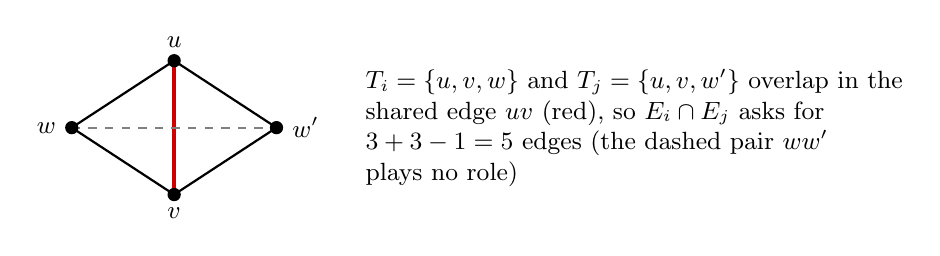
\begin{tikzpicture}[thick, every node/.style={font=\small}]
        \coordinate (c) at (0,0);
        \coordinate (a) at (1.3,0.85);
        \coordinate (b) at (1.3,-0.85);
        \coordinate (d) at (2.6,0);
        \draw (c) -- (a) (c) -- (b) (a) -- (d) (b) -- (d);
        \draw[red!80!black, line width=1.4pt] (a) -- (b);
        \draw[gray, dashed] (c) -- (d);
        \foreach \p in {a,b,c,d} \fill (\p) circle (2.4pt);
        \node[above=1pt] at (a) {$u$};
        \node[below=1pt] at (b) {$v$};
        \node[left=2pt] at (c) {$w$};
        \node[right=2pt] at (d) {$w'$};
        \node[anchor=west, align=left] at (3.6,0)
            {$T_i = \{u,v,w\}$ and $T_j = \{u,v,w'\}$ overlap in the\\shared edge $uv$ (red), so $E_i \cap E_j$ asks for\\$3 + 3 - 1 = 5$ edges (the dashed pair $ww'$\\plays no role)};
    \end{tikzpicture}
\end{center}

\emph{How many.} Such a pair of triples, taken unordered, is determined by its \(4\) vertices together with which of the \(6\) pairs among them is the shared edge, and conversely each such choice gives one. So there are \(6\binom{n}{4}\) of them, hence \(12\binom{n}{4} = \Theta(n^{4})\) ordered pairs \((i,j)\) with \(i \sim j\).

\emph{With what probability.} As the picture shows, \(E_i \cap E_j\) asks for \(3 + 3 - 1 = 5\) distinct edges, so \(\mathbb{P}(E_i \cap E_j) = p^{5}\).

Putting the three together,
\[
    \Delta = \sum_{i \sim j} \mathbb{P}(E_i \cap E_j) = 12\binom{n}{4} p^{5} = \Theta\bigl( n^{4} p^{5} \bigr).
\]

\begin{proposition}\label{prop:triangle-dense}
    If \(p \gg \frac{1}{n}\), then with high probability \(G(n,p)\) has \((1+o(1)) \binom{n}{3}p^{3} \to \infty\) triangles; in particular it has a triangle.
\end{proposition}

\begin{proof}
    We have \(\mathbb{E}[X] = \Theta\bigl( n^{3}p^{3} \bigr) \to \infty\), and with \(\Delta = \Theta(n^{4}p^{5})\) from above,
    \[
        \frac{\Delta}{\mathbb{E}[X]^{2}} = \Theta\Bigl( \frac{n^{4}p^{5}}{n^{6}p^{6}} \Bigr) = \Theta\Bigl( \frac{1}{n^{2}p} \Bigr) = o(1),
    \]
    the last step because \(n^{2}p = n \cdot (np) \to \infty\). So \(\Delta = o\bigl( \mathbb{E}[X]^{2} \bigr)\) and \autoref{cor:second-moment} applies.
\end{proof}

\subsection{Summary}

\begin{theorem}\label{thm:triangle-threshold}
    Let \(X\) be the number of triangles in \(G(n,p)\). Then, with high probability,
    \[
        X = \begin{cases}
            0, & \text{if } p \ll \frac{1}{n}, \\[2pt]
            (1+o(1)) \dfrac{(np)^{3}}{6} \to \infty, & \text{if } p \gg \frac{1}{n}.
        \end{cases}
    \]
\end{theorem}

So \(p = \frac{1}{n}\) is a \vocab{threshold} for containing a triangle: on one side the property fails with high probability, on the other it holds with high probability.
\begin{center}
    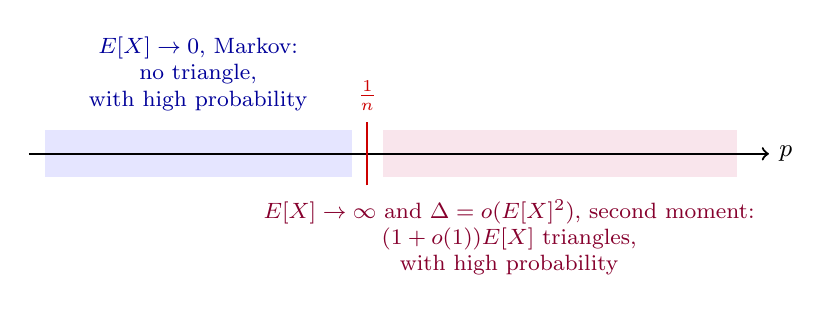
\begin{tikzpicture}[thick, every node/.style={font=\small}]
        \fill[blue!10] (0.2,-0.3) rectangle (4.1,0.3);
        \fill[purple!10] (4.5,-0.3) rectangle (9.0,0.3);
        \draw[->] (0,0) -- (9.4,0) node[right] {$p$};
        \draw[red!80!black] (4.3,-0.4) -- (4.3,0.4);
        \node[red!80!black, anchor=south] at (4.3,0.42) {$\frac{1}{n}$};
        \node[blue!60!black, anchor=south, align=center, font=\footnotesize] at (2.15,0.42)
            {$\mathbb{E}[X] \to 0$, Markov:\\no triangle,\\with high probability};
        \node[purple!70!black, anchor=north, align=center, font=\footnotesize] at (6.1,-0.45)
            {$\mathbb{E}[X] \to \infty$ and $\Delta = o(\mathbb{E}[X]^2)$, second moment:\\$(1+o(1))\mathbb{E}[X]$ triangles,\\with high probability};
    \end{tikzpicture}
\end{center}

\begin{remark}\hfill
    \begin{enumerate}[(1)]
        \item The threshold is where \(\mathbb{E}[X]\) itself changes behavior, namely where \(n^{3}p^{3}\) crosses a constant. This is not an accident, and identifying thresholds by computing a first moment and then controlling the second is the standard route.
        \item It is worth looking back at \autoref{thm:erdos-girth} with this in hand. There we took \(p = n^{\theta-1}\) with \(\theta > 0\), which is \emph{above} the threshold, so that random graph contains \(\Theta(n^{3\theta})\) triangles with high probability --- it is nowhere near triangle-free. The alteration was unavoidable; what made it work was not that the short cycles were absent but that there were \(o(n)\) of them.
        \item The regime \(p = \frac{c}{n}\) is left open here. There \(\mathbb{E}[X] \to \frac{c^{3}}{6}\), a constant, and the number of triangles converges to a Poisson distribution rather than concentrating; neither \thmref{thm:markov} nor \autoref{cor:second-moment} settles it.
    \end{enumerate}
\end{remark}
